\documentclass{article}
\usepackage{graphicx}

\begin{document}

\begin{titlepage}
\title{ECS189G Term Project Report Problem A}
\author{Goh Chang Kang, Charles 916751838 ccgoh@ucdavis.edu, \\
Yang Minxing 916751773 mixyang@ucdavis.edu, \\ 
Chen Jieyi Chloe 999823783 eyichen@ucdavis.edu}

\date{December 8, 2018}
\maketitle
\end{titlepage}

\tableofcontents
\pagebreak

\section{Introduction}

We are given a data set detailing the votes of USA's house of 
representativess on various issues. Some of the votes are marked with a "?", 
indicating that the representatives did not vote for those cases. Our objective
is to predict their votes. The table below shows the breakdown of the support
Democrats and Republicans gave to each topic before predicting any of the votes: \newline

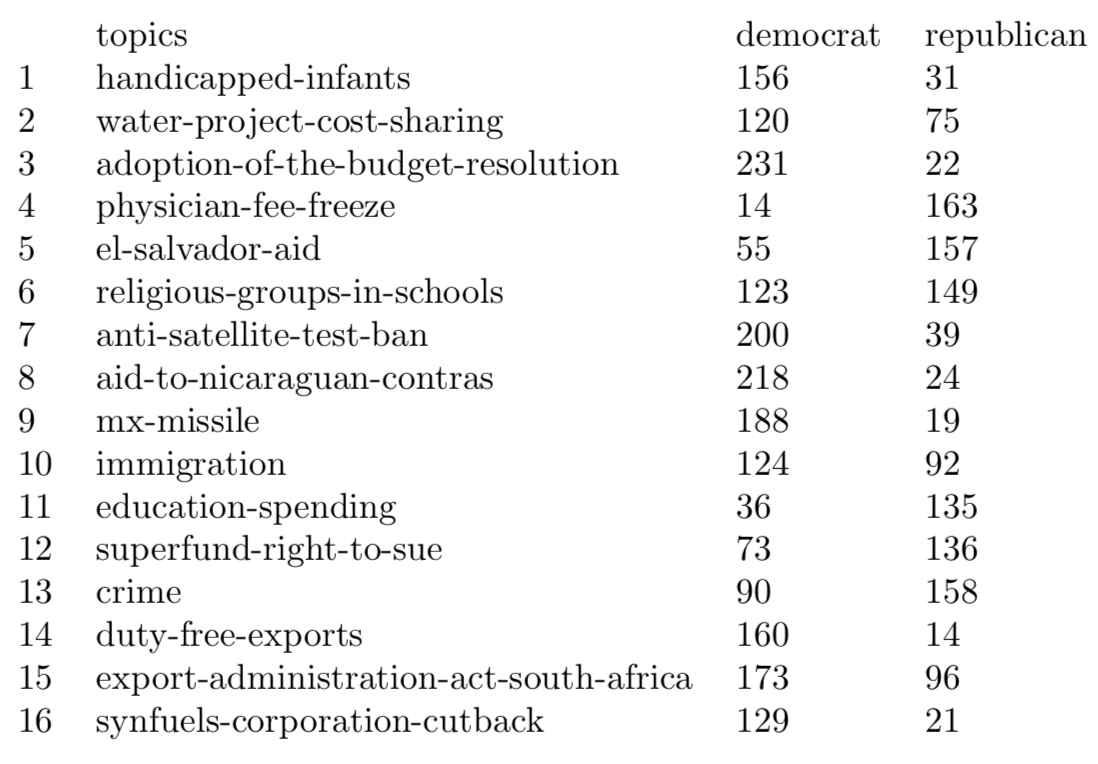
\includegraphics[scale=0.5]{starting_votes.png}

\subsection{Overview of Terminology}
\subsubsection{k Nearest Neighbours}
K Nearest Neighbor is a method that finds the average rating of the k similar users to a 
given individual to form a predicted rating for that individual.

\subsubsection{Non-negative Matrix Factorization}
Non-negative matrix factorizaiton is a feature extraction method that 
factorized a matrix A into two smaller matrices W and H where A is the
input data matrix with users and features information. The 
dot product of W and H would give the approximate predictions of A. 

\subsubsection{Latent Factor Model}
Latent Factor Model takes the user and item effect into consideration when doing predictions. 

\subsubsection{Probability of Guessing Correctly}
PGEC = Number of Correct Prediction/Total Number of Observations \newline

\section{Method}

For ease of use, we named the columns of 
the different issues based on the side information provided by the database.
We can determine that the dataset can be represented by 1s and 0s for ease of data analysis
since the house representative can only be categorically classified by 2 parties and can either vote
yes or no (or not at all).
By reformatting the dataset, we obtain one from which we can easily process, train and 
predict. This is a short extract from the newly formatted dataset:

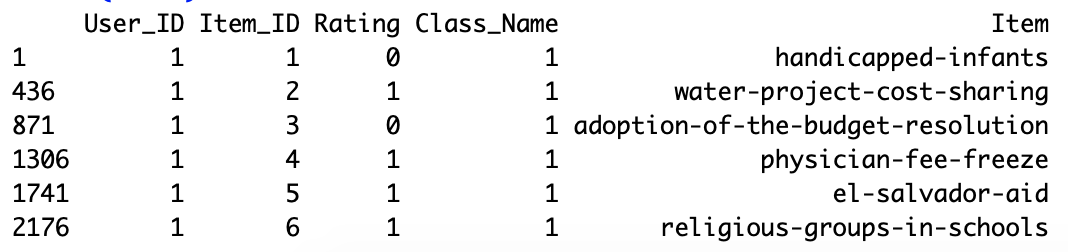
\includegraphics[scale=0.6]{raw_data_example.png}
\linebreak
By examining the dataset, we notice that there are many instances where the
house representatives did not vote. These entries are marked by a "?". Our objective
is to predict their votes. In order to train our predictor model, we split the dataset
into one with no missing votes and one with missing votes.
There are a number of ways to train our predictor model. For this dataset we have
decided to test the accuracy of using K nearest neighbours, Non-Negative matrix 
factorization and Latent Factor Model. To decide on the best model, we test the 3 models before predicting using the Probability of Guessing Correctly (the closer to
1 the better). 

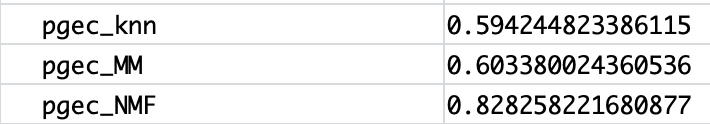
\includegraphics[scale=0.85]{accuracy_test_problemA.png}
\linebreak
We can see that the PGEC for non-Negative Matrix factorization gives the highest
accuracy and therefore conclude that it is the best model to use in the prediction
of the missing votes. We can then decide to train the model using non-Negative Matrix 
factorization before predicting the missing votes.
\linebreak
Doing so, we have predicted the votes for politicians who did not vote in a
particular issue. Here is an extract of the predicted votes using non-Negative Matrix factorization
(where 1 corresponds to a yes, and 0 corresponds to a no):

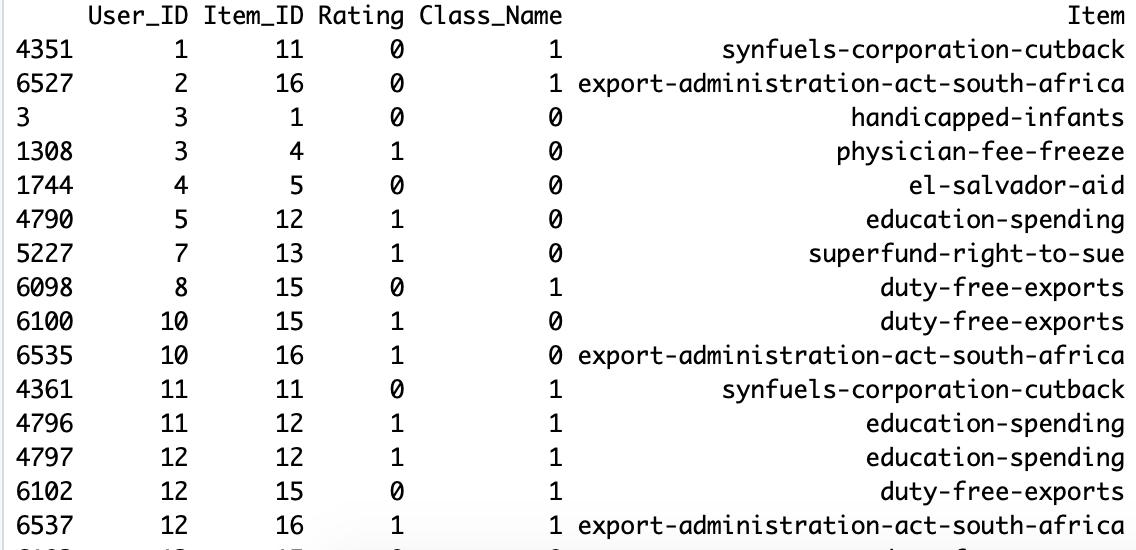
\includegraphics[scale=0.5]{prediction_results_problemA.png}

\section{Discussion}

We can combine known votes with predicted votes to get a full picture of what
the votes would be like as if everyone voted for everything:
\linebreak
Out of interest, we can also produce a table to show the number of votes that
democrat and republican representatives voted for and were predicted to vote for
for different issues. We can see that the general trend remains in the votes, i.e. if
more democrats voted in favour of an issue in the original dataset then more democrats will tend 
to vote in favour of the issue in the dataset with predicted data and original data. 

\pagebreak

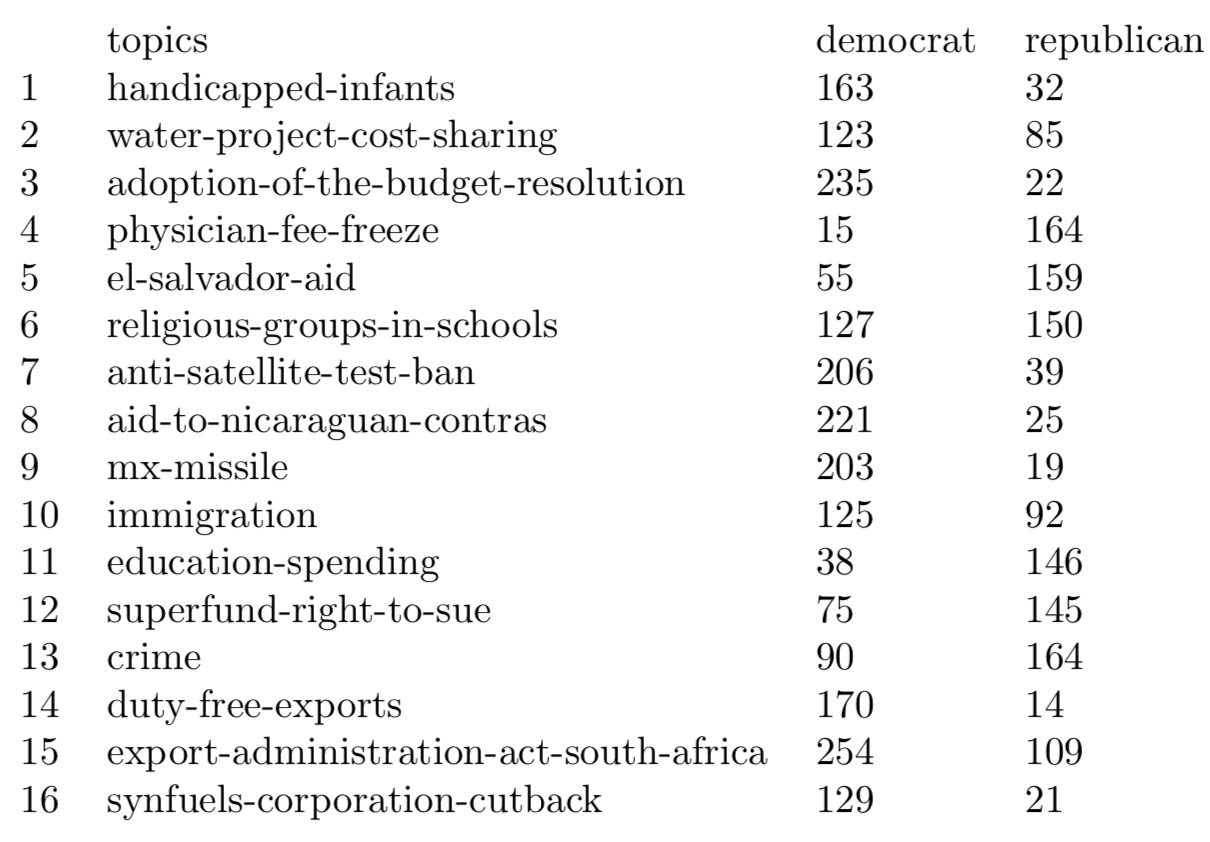
\includegraphics[scale=0.5]{ending_votes.png}

\section{Author Contributions}
All group members contributed equally in this project.

\section{Appendix}
The following code was used for this problem:
\begin{verbatim}
  # Problem 1
  house_vote = read.table('house-votes-84.data', sep = ',')
  names(house_vote) = c('Class Name', 'handicapped-infants', 
      'water-project-cost-sharing', 'adoption-of-the-budget-resolution',
      'physician-fee-freeze', 'el-salvador-aid', 
      'religious-groups-in-schools', 'anti-satellite-test-ban',
      'aid-to-nicaraguan-contras', 'mx-missile', 'immigration', 
      'synfuels-corporation-cutback', 'education-spending', 
      'superfund-right-to-sue', 'crime', 'duty-free-exports', 
      'export-administration-act-south-africa')

  # display the unique items in each column
  apply(house_vote, 2, unique)

  # Use nearest neighbor, matrix factorization, hybrid model 
  (nearest neighbor and matrix factorization)
  library(rectools)

  # UserID = members of Congress
  # Movie ID = legislative bills 
  # Rating = votes
  as.numeric(as.factor(house_vote$`Class Name`))

  # check whether each column in house_vote is factor
  col_index <- sapply(house_vote, is.factor)

  house_vote_factor = data.frame(matrix(NA, ncol = ncol(house_vote), 
    nrow = nrow(house_vote)))
  house_vote_factor

  # replace ? with NA value
  house_vote[house_vote == '?'] = NA

  # 1 for yes, 0 for non-yes
  # 1 for republicans, 0 for democrats
  house_vote_factor[col_index] <- lapply(house_vote[col_index], 
    function(x) c(0, 1)[as.numeric(as.factor(as.vector(x)))])

  house_vote_factor
  # change the column name into numeric
  names(house_vote_factor) = seq(1, ncol(house_vote), by = 1)

  names(house_vote_factor) = names(house_vote)

  colnames(house_vote_factor)

  # check how many missing_vote we need to predict
  table(is.na(house_vote_factor))

  library(rectools)
  # stack the columns so that it has the required format to 
  # input into the formUserData function
  house_final = cbind(house_vote_factor[1], stack(house_vote_factor
    [2: ncol(house_vote_factor)]))
  names(house_final) = c('Class_Name', 'Rating', 'Item')
  house_final$User_ID = rep(1:nrow(house_vote_factor), times = 
    nrow(house_final)/nrow(house_vote_factor))
  house_final$Item_ID = as.numeric(as.factor(house_final$Item))
  house_final = house_final[c('User_ID', 'Item_ID', 'Rating', 'Class_Name', 'Item')]

  house = house_final[order(house_final$User_ID), ]

  # create a dataframe to store user and item information with nan value
  house_nan = house[is.na(house$Rating), ]
  # remove na value from the dataframe
  house = na.omit(house)
  # reset index
  rownames(house) = NULL

  # See voting trends for politicians who did vote
  topics <- unique(house[,5])
  items <- c()
  democrat <- c()
  republican <- c()
  lapply(topics, function(x) {
    democrat <<- c(democrat, length(which(house$Class_Name == 0 
      & house$Rating == 1 & house$Item == x)))
    republican <<- c(republican, length(which(house$Class_Name == 1 
      & house$Rating == 1 & house$Item == x)))
  })
  topic_by_party_analysis_not_predicted <- cbind.data.frame(topics, 
    democrat, republican)
  write.csv(topic_by_party_analysis_not_predicted, 
    "topic_by_party_analysis_not_predicted.csv")

  # form the user
  form_house = formUserData(house[, 1:3], usrCovs = house[4])
  # test with one user
  predict.usrData(form_house, form_house[[10]], 11, 10, wtcovs = 1)

  # get the ratings for all users with nan ratings
  nrow(house_nan)

  datum = list(userID = house_nan$User_ID, 
    itms = house_nan$Item_ID, ratings = house_nan$Rating)


  # Edited KNN Function
  predict_knn = function(user_id, item_id) {
    usrRatings = house[which(house$User_ID == user_id), ]$Rating
    datum = list(userID = user_id,itms = item_id, ratings=usrRatings)
    knn_output = predict.usrData(origData = form_house, datum, item_id, k = 10)
    
    if (knn_output >= 0.5) {
      return (1)
    }
    else{
      return(0)
    }
  }

  house_output = mapply(predict_knn, house$User_ID, house$Item_ID)
  actual_ratings = house['Rating']
  final_df = cbind(actual_ratings, house_output)
  pgec_knn = nrow(final_df[final_df['Rating'] 
    == final_df['house_output'], ])/nrow(final_df)

  ## Matrix Factorization
  trn = trainReco(house[, 1:3], nmf = TRUE)
  # since predict.RecoS3 does not return a categorical variable, we need to 
  # add a condition
  ### Option 1: member = 249 does not vote anyone, give a message to the user
  predict_mf = function(user_id, item_id){
    # if the rating value >= 0.5, rating is y, else is n
    onerec = data.frame(matrix(nrow = 1, ncol = 2))
    names(onerec) = c('User_ID', 'Item_ID')
    onerec$User_ID = user_id
    onerec$Item_ID = item_id
    if (is.na(predict.RecoS3(trn, onerec))) {
      return ('This politician does not vote for any bill in the past')
    }
    else if (predict.RecoS3(trn, onerec) >= 0.5){
      return (1)
    }
    else {
      return(0)
    }
  }

  # since predict.RecoS3 does not return a categorical variable, 
  # we need to add a condition
  #### Option 2: member = 249 does not vote anyone, set it to 0
  predict_mf = function(user_id, item_id){
    # if the rating value >= 0.5, rating is y, else is n
    onerec = data.frame(matrix(nrow = 1, ncol = 2))
    names(onerec) = c('User_ID', 'Item_ID')
    onerec$User_ID = user_id
    onerec$Item_ID = item_id
    if ((predict.RecoS3(trn, onerec) < 0.5) | 
      (is.na(predict.RecoS3(trn, onerec)))){
      return (0)
    }
    else {
      return(1)
    }
  }

  # Get PGEC value for NMF
  house_output = mapply(predict_mf, house$User_ID, house$Item_ID)
  actual_ratings = house['Rating']
  final_df = cbind(actual_ratings, house_output)
  pgec_NMF = nrow(final_df[final_df['Rating'] 
    == final_df['house_output'], ])/nrow(final_df)

  # Method of momments
  mmout <- trainMM(house[,1:3])
  prediction <- predict(mmout, house[,1:2])
  prediction <- sapply(prediction, function(x) {
    if (x < 0.5) {
      x <- 0
    } else {
      x <- 1
    }
  })
  final_df <- cbind(house, prediction)
  pgec_MM = nrow(final_df[final_df['Rating'] 
    == final_df['prediction'], ])/nrow(final_df)

  # Prediction of NaN values using KNN
  knn_result = mapply(predict_knn, house_nan$User_ID, house_nan$Item_ID)

  # Predition of NaN values using NMF
  mf_result = mapply(predict_mf, house_nan$User_ID, house_nan$Item_ID)

  # Prediction of NaN values using MM
  mm_result = predict(mmout, house_nan[, 1:2])

  # Votes That Were Unprocessed and Used to Train Model
  house

  # Votes That were Predicted after training model using Matrix Factorization
  predicted_results_with_mf <- house_nan
  predicted_results_with_mf$Rating <- mf_result
  predicted_results_with_mf

  # All data: predicted and non-predicted together
  library(dplyr)
  result <- bind_rows(house, predicted_results_with_mf)

  topics <- unique(result[,5])

  items <- c()
  democrat <- c()
  republican <- c()
  lapply(topics, function(x) {
    democrat <<- c(democrat, length(
      which(result$Class_Name == 0 & result$Rating == 1 & result$Item == x)))
    republican <<- c(republican, length(
      which(result$Class_Name == 1 & result$Rating == 1 & result$Item == x)))
  })
  topic_by_party_analysis_altogether <- cbind.data.frame(topics, democrat, republican)
  write.csv(topic_by_party_analysis_altogether, 
  "topic_by_party_analysis_altogether.csv")
\end{verbatim}

\begin{thebibliography}{1}

  \bibitem{rsbook} Norman Matloff {\em A Tour of Recommender Systems}  2018.

\end{thebibliography}

\end{document}